\documentclass{beamer}
\usetheme{metropolis}
% =========================================================================
% Preamble (adapted from group's house style)
% =========================================================================
\setbeamercolor{titlelike}{parent=structure,bg=cyan}
\usepackage{graphicx}
\graphicspath{{figures/}}
\usepackage{amsmath}
\usepackage{amssymb}
\usepackage{booktabs}
\setbeamerfont{title}{size=\fontsize{15}{16}\selectfont}

\makeatletter
\usepackage{soul}
\setlength{\metropolis@titleseparator@linewidth}{1.1pt}
\setlength{\metropolis@progressonsectionpage@linewidth}{1.1pt}
\setlength{\metropolis@progressinheadfoot@linewidth}{1.1pt}
\makeatother
\usepackage[font=footnotesize]{caption}

\usepackage{tcolorbox}
\tcbuselibrary{skins}
\tcbset{
    minimaliststyle/.style={
        enhanced,
        colback=blue!6,
        boxrule=1pt,
        sharp corners,
        left=2mm, right=2mm, top=3mm, bottom=4mm,
        before=\vspace{1mm}, after=\vspace{0.8mm}
    }
}
\newcommand{\highlightbox}[1]{
    \begin{tcolorbox}[minimaliststyle]
        #1
    \end{tcolorbox}
}

\AtBeginDocument{\fontsize{8}{10}\selectfont}

\setbeamercolor{background canvas}{bg=white}
\setbeamercolor{title separator}{fg=blue!50!black}
\setbeamerfont{title separator}{size=\Large}
\setbeamercolor{progress bar}{fg=blue!50!black}
\setbeamercolor{frametitle}{bg=blue!55!black, fg=white}
\setbeamercolor{itemize item}{fg=blue!30!black}

\usepackage{pifont}
\setbeamertemplate{itemize item}{\fontsize{7}{9}\selectfont\ding{118}}
\setbeamertemplate{itemize subitem}{\fontsize{6}{8}\selectfont\ding{118}}

\usepackage{hyperref}
\setbeamertemplate{navigation symbols}{}
\setbeamertemplate{footline}[frame number]
\setbeamertemplate{caption}[numbered]
\vspace*{-1.8cm}

% =========================================================================
% Title
% =========================================================================
\title{Overworked Americans\\[0.3em]\large Problem 1: Q1, Q4, Q5, Q7}
\setbeamerfont{author}{size=\scriptsize}
\author{Alessandro Caggia \and Stefano De Bianchi \and Eduard Hartel \and Francesco Mastidoro}
\setbeamerfont{date}{size=\tiny}
\date{Take-Home, Advanced Microeconomics (20296) --- May 2026}

\begin{document}

\begin{frame}
    \titlepage
\end{frame}

% =========================================================================
% Footer styling
% =========================================================================
\setbeamercolor{author in head/foot}{bg=blue!55!black, fg=white}
\setbeamercolor{title in head/foot}{bg=white, fg=blue!55!black}
\setbeamercolor{date in head/foot}{bg=white, fg=blue!55!black}

\setbeamertemplate{footline}{
    \leavevmode%
    \hbox{
        \begin{beamercolorbox}[wd=.33\paperwidth,ht=2.5ex,dp=1ex,left]{author in head/foot}%
            \hspace{1em} Caggia / De Bianchi / Hartel / Mastidoro
        \end{beamercolorbox}%
        \begin{beamercolorbox}[wd=.33\paperwidth,ht=2.5ex,dp=1ex,center]{title in head/foot}%
            Overworked Americans
        \end{beamercolorbox}%
        \begin{beamercolorbox}[wd=.33\paperwidth,ht=2.5ex,dp=1ex,right]{date in head/foot}%
            Slide \insertframenumber{} of \inserttotalframenumber \hspace{1em}
        \end{beamercolorbox}}%
    \vskip0pt%
}

% =========================================================================
\section{Q1 --- Documenting the EU--US hours gap}
% =========================================================================

% -------------------------------------------------------------------------
% Q1, Slide 1: Question and roadmap
% -------------------------------------------------------------------------
\begin{frame}{Q1 --- Question and roadmap}
\textit{``Document the EU--US (and intra-EU) hours-worked gap in recent years.''}

\vspace{0.5em}
\textbf{What we deliver.}
\begin{itemize}\setlength{\itemsep}{6pt}
    \item One stylised fact (three panels): hours fell, the tax wedge does not cleanly explain the cross-section.
    \item Two questions panel (c) raises:
        \begin{itemize}
            \item \textbf{(I)} the true slope of the tax--hours relation;
            \item \textbf{(II)} the wide \emph{residual scatter} around it ($\sigma_{\rm resid}\!\approx\!158$ hours).
        \end{itemize}
    \item Q4 (cap) and Q5 (union bargaining) develop two institutional channels that sit in those residuals as endogenous confounders.
\end{itemize}

\vspace{0.3em}
\textbf{Decomposition.} For the working-age (15--64) population, $H/N = HE\cdot e$. Bick--Br\"uggemann--Fuchs-Sch\"undeln (2019) attribute roughly half of the EU--US gap to each margin. We focus on $HE$ (intensive margin) --- the prompt asks about hours.
\end{frame}

% -------------------------------------------------------------------------
% Q1, Slide 2: The fact (figure)
% -------------------------------------------------------------------------
\begin{frame}{Q1 --- The fact}
\begin{figure}
    \centering
    
\includegraphics[width=0.96\linewidth]{figure_panel.pdf}
    \caption{(a) Hours per worker, \% deviation from US, 1970--2024. (b) Effective labour wedge $\tau_h$, \% deviation, 1970--2007. (c) OECD labour-tax wedge vs hours per worker, 2023 cross-section ($n\!=\!19$); OLS line and $\pm 1\sigma_{\rm resid}$ band.}
\end{figure}
\end{frame}

% -------------------------------------------------------------------------
% Q1, Slide 3: Three readings of the panel
% -------------------------------------------------------------------------
\begin{frame}{Q1 --- Three readings of the panel}
\begin{itemize}\setlength{\itemsep}{8pt}
    \item \textbf{(i) Hours fell relative to US since 1970:} DE/NL $\approx\!-25$ to $-30\%$; IT/ES $\approx\!-10$ to $-15\%$.
    \item \textbf{(ii) Wedge cross-country pattern is unstructured:} Italy's relative wedge drifts up, the UK's narrows, France stays flat. No clean mirroring of panel-(a) hours.
    \item \textbf{(iii) The 2023 cross-section is signed correctly but noisy:} OLS slope $-9.9$ hrs/pp, $R^{2}\!=\!0.16$, residual SD $\approx\!158$ hours $\approx$ a third of the entire DE--US gap. Italy (45.1\%) and Greece (36.7\%) work \emph{more} than France (46.8\%); the four highest-$\tau$ countries (BE, DE, AT, FR) span $\approx\!200$ hours within a 6\,pp wedge band.
\end{itemize}

\vspace{0.3em}
\textbf{Bottom line.} Tax wedges sign the relation correctly but cannot pin its slope (endogenous $\tau$) and cannot account for the scatter. Q4 and Q5 are not orthogonal additions to the tax effect: they live in the residuals as endogenous confounders.
\end{frame}

% =========================================================================
\section{Q4 --- Hours regulation: optimality of a cap}
% =========================================================================

% -------------------------------------------------------------------------
% Q4, Slide 1: Setup and three bliss points
% -------------------------------------------------------------------------
\begin{frame}{Q4 --- Setup: three bliss points and the firm-power ordering}
\textbf{Primitives} (quadratic-disutility worker, linear-quadratic firm):
\[
V_w(h)=(1\!-\!\tau)wh-\tfrac{\alpha}{2}h^{2},\qquad V_f(h)=Ah-\tfrac{\beta}{2}h^{2}-wh.
\]
Wage transfer cancels in $W\!=\!V_w\!+\!V_f$. Three FOCs give three bliss points:
\[
h^{*}=\frac{(1\!-\!\tau)w}{\alpha},\quad
h^{\mathrm{soc}}=\frac{A-\tau w}{\alpha+\beta},\quad
h^{\mathrm{firm}}=\frac{A-w}{\beta}.
\]

\textbf{Cap as quantity instrument.} The firm picks $h$ to maximise $V_f$ s.t.\ $h\!\le\!\bar h$, with $w$ pinned by IR $V_w(h)\!=\!V_w^{0}$. KKT yields $h^{\mathrm{eq}}(\bar h)\!=\!\min\{\bar h,\,h^{\mathrm{firm}}\}$.

\vspace{0.3em}
\textbf{Firm-power ordering.} At baseline $(A,w,\tau,\alpha,\beta)\!=\!(2,1,0.4,2,2)$:
\[
h^{*}=0.30\;<\;h^{\mathrm{soc}}=0.40\;<\;h^{\mathrm{firm}}=0.50.
\]
The firm overshoots the social optimum: a binding cap has something to correct.
\end{frame}

% -------------------------------------------------------------------------
% Q4, Slide 2: Optimality condition for the cap
% -------------------------------------------------------------------------
\begin{frame}{Q4 --- Optimality condition for the cap}
\textbf{Three surpluses} (relative to the no-cap baseline $h^{\mathrm{firm}}$):
\begin{align*}
\Delta V_f(\bar h) &= -\tfrac{\beta}{2}\bigl(h^{\mathrm{firm}}-\bar h\bigr)^{2}\;\le\;0, \\
\Delta W(\bar h)   &= -\tfrac{\alpha+\beta}{2}\!\left[(h^{\mathrm{soc}}-\bar h)^{2}-(h^{\mathrm{soc}}-h^{\mathrm{firm}})^{2}\right].
\end{align*}

\textbf{Welfare condition} ($W$ is symmetric in $\bar h$ around $h^{\mathrm{soc}}$):
\[
\Delta W(\bar h)>0\;\;\Longleftrightarrow\;\;\bar h\in\bigl(\,2h^{\mathrm{soc}}-h^{\mathrm{firm}},\;h^{\mathrm{firm}}\,\bigr).
\]
Peak at $\bar h=h^{\mathrm{soc}}$ with gain $\tfrac{\alpha+\beta}{2}(h^{\mathrm{firm}}-h^{\mathrm{soc}})^{2}=0.020$ at calibration.

\vspace{0.3em}
\textbf{Optimality condition.} The cap is welfare-improving \emph{iff} it pulls hours toward $h^{\mathrm{soc}}$ without overshooting; it destroys joint surplus when $\bar h<2h^{\mathrm{soc}}-h^{\mathrm{firm}}$ (firm losses dominate). At $\alpha\!=\!\beta$ the lower band edge collapses to $h^{*}\!=\!0.30$.
\end{frame}

% -------------------------------------------------------------------------
% Q4, Slide 3: Simulation figure
% -------------------------------------------------------------------------
\begin{frame}{Q4 --- Simulation: welfare gain over the cap}
\begin{figure}
    \centering
    
\includegraphics[width=0.99\linewidth]{sim_cap.pdf}
    \caption{(a) Primitives $V_w,V_f,W$ over $h$ with bliss points marked. (b) Surpluses along $h^{\mathrm{eq}}(\bar h)\!=\!\min\{\bar h,h^{\mathrm{firm}}\}$. (c) $\Delta W(\bar h)$ vs no-cap baseline; \textbf{green} = welfare-improving band, \textbf{red} = overshoot. Peak gain $\Delta W\!=\!0.020$ at $\bar h\!=\!h^{\mathrm{soc}}\!=\!0.40$.}
\end{figure}
\end{frame}

% -------------------------------------------------------------------------
% Q4, Slide 4: Reading + empirical anchor
% -------------------------------------------------------------------------
\begin{frame}{Q4 --- Two thresholds and the Aubry anchor}
\textbf{Two distinct thresholds} as the cap tightens past $h^{\mathrm{soc}}$:
\begin{itemize}\setlength{\itemsep}{6pt}
    \item Joint surplus turns negative once $\bar h<2h^{\mathrm{soc}}-h^{\mathrm{firm}}\!=\!0.30$ (firm losses dominate worker gains).
    \item The individual worker still benefits until $\bar h\!=\!h^{*}\!=\!0.30$, and only becomes worse off than no-cap at $\bar h<2h^{*}-h^{\mathrm{firm}}\!=\!0.10$.
    \item For $\bar h\!\in\!(0.10,\,0.30)$: \emph{cap reduces aggregate welfare but the worker still gains}.
\end{itemize}

\vspace{0.3em}
\textbf{Empirical anchor (Aubry, France 1998--2000).} Estev\~ao--S\'a (2008): $\approx\!10$--$13\%$ hours cut, near-zero employment effect. Consistent with a binding cap at $\bar h/h^{\mathrm{firm}}\!\approx\!0.875$, well \emph{inside} the welfare-improving band.
\end{frame}

% =========================================================================
\section{Q5 --- A single union as welfare-restorer}
% =========================================================================

% -------------------------------------------------------------------------
% Q5, Slide 1: RTM Nash bargain reduces to a quadratic
% -------------------------------------------------------------------------
\begin{frame}{Q5 --- Right-to-manage Nash bargain}
\textbf{Setup.} Single encompassing union (Calmfors--Driffill 1988); on the firm's labour demand $h^d_j(w)\!=\!(A_j-w)/\beta$, with $x_j\!\equiv\!A_j-w$:
\[
V_w(x_j)=A_v x_j-B_v x_j^{2},\qquad V_f(x_j)=\frac{x_j^{2}}{2\beta},
\]
$A_v\!\equiv\!(1\!-\!\tau)A_j/\beta$, $B_v\!\equiv\!(1\!-\!\tau)/\beta+\alpha/(2\beta^{2})$.

\textbf{Bargain.} Union and firm pick $w$ via asymmetric Nash with worker weight $\eta\!\in\![0,1]$:
\[
\max_{w}\;\bigl[V_w(w;A_j)-V_w^{0}\bigr]^{\eta}\,V_f(w;A_j)^{1-\eta}.
\]
Interior FOC reduces to a quadratic in $x_j$:
\[
2B_v\,x_j^{2}-A_v(2-\eta)\,x_j+2(1-\eta)\,V_w^{0}=0.
\]
\textbf{Larger root} $x_j^{\star}(\eta)$ delivers $w_j(\eta)=A_j-x_j^{\star}$, $h_j(\eta)=x_j^{\star}/\beta$.

\vspace{0.3em}
\textbf{Boundaries.} $\eta\!=\!0$: IR binds ($V_w\!=\!V_w^0$), $h_j\!=\!h^{\mathrm{firm}}_j$. $\eta\!\to\!1$: $x^\star_j(1)\!=\!A_v/(2B_v)$, $h_j(1)\!<\!h^*(w_j(1))$.
\end{frame}

% -------------------------------------------------------------------------
% Q5, Slide 2: Comparative statics + welfare-restorer
% -------------------------------------------------------------------------
\begin{frame}{Q5 --- Comparative statics and the welfare-restorer}
\textbf{Implicit differentiation} of the bargain quadratic in $\eta$:
\[
\bigl[\,4B_v x_j-A_v(2-\eta)\,\bigr]\frac{dx_j}{d\eta}=-A_v x_j+2V_w^{0}.
\]
Bracket on LHS = $\sqrt{D(\eta)}\!>\!0$ on $[0,1]$ under (R1) $A_v^{2}\!>\!4B_vV_w^0$.
RHS strictly negative since $A_v x^\star_j\!\ge\!A_v^{2}/(2B_v)\!>\!2V_w^0$ (also (R1)). So:
\[
\frac{dx_j}{d\eta}<0,\qquad \frac{dw_j}{d\eta}>0,\qquad \frac{dh_j}{d\eta}<0.
\]

\textbf{Welfare-restorer.} $W$ concave with peak at $h^{\mathrm{soc}}_j\!\in\!(h^*_j,h^{\mathrm{firm}}_j)$. Since $h_j(\eta)$ is continuous and strictly decreasing with $h_j(0)\!=\!h^{\mathrm{firm}}_j$, IVT gives a unique $\hat\eta_j\!\in\!(0,1)$ with $h_j(\hat\eta_j)\!=\!h^{\mathrm{soc}}_j$:
\[
W(h_j(\eta))-W(h^{\mathrm{firm}}_j)=-\tfrac{\alpha+\beta}{2}\!\left[(h^{\mathrm{soc}}_j\!-\!h_j(\eta))^{2}-(h^{\mathrm{soc}}_j\!-\!h^{\mathrm{firm}}_j)^{2}\right]
\]
increasing on $[0,\hat\eta_j]$, decreasing thereafter (overshoot logic of Q4).

\vspace{0.3em}
\textbf{Calibration.} OECD ICTWSS coverage maps US ($\sim\!12\%$) to $\eta^{\,US}\!\approx\!0.15$; EU ($\sim\!60$--$70\%$) to $\eta^{\,EU}\!\approx\!0.5$. EU--US hours gap $\approx\!0.08$ ($\approx\!19\%$ logs).
\end{frame}

% -------------------------------------------------------------------------
% Q5, Slide 3: Sectoral shocks figure
% -------------------------------------------------------------------------
\begin{frame}{Q5 --- Sectoral shocks: pass-through and asymmetry}
\begin{figure}
    \centering
    
\includegraphics[width=0.99\linewidth]{sim_shocks.pdf}
    \caption{Mean-preserving sectoral shock $A_g\!=\!2.2,\,A_b\!=\!1.8$ at $\eta\!=\!0.5$. (a) Demand shifts and equilibria; rigid bad-sector at stuck $w_{\rm pre}$. (b) Hours: bad-sector rigid is $36\%$ below FM. (c) Firm profit: bad-sector rigid is $60\%$ below FM.}
\end{figure}
\end{frame}

% -------------------------------------------------------------------------
% Q5, Slide 4: Asymmetric pass-through under wage rigidity
% -------------------------------------------------------------------------
\begin{frame}{Q5 --- Asymmetric pass-through under wage rigidity}
\textbf{Flexible union ($A_g\!=\!2.2,\,\eta\!=\!0.5$).} $w_g^U\!=\!1.354,\,h_g^U\!=\!0.423$. Productivity gain splits into wages ($\Delta w/w\!=\!+25\%$) and reduced hours ($\Delta h/h\!=\!-24\%$); joint surplus falls only $\approx\!5\%$ ($W^{\rm FM}_g\!=\!0.363\!\to\!W^U_g\!=\!0.344$). \textbf{Bulk of redistribution = wage-rent transfer, not deadweight loss.}

\vspace{0.3em}
\textbf{Rigid bad sector ($A_b\!=\!1.8$, $w$ stuck at $w_{\rm pre}\!=\!1.242$).} Hours read off labour demand at the stuck wage:
\[
h_b^{\rm rig}=(A_b-w_{\rm pre})/\beta=0.279.
\]
Hours $-36\%$ vs FM, profit $-60\%$ vs FM.

\vspace{0.3em}
\textbf{Headline.}
\begin{itemize}\setlength{\itemsep}{4pt}
    \item Good shocks pass through \emph{diluted}: absorbed in wage rents.
    \item Bad shocks pass through \emph{amplified}: rigidity forces hours to absorb the entire shock.
\end{itemize}

\vspace{0.2em}
The encompassing-union setup $+$ downward wage rigidity makes the channel asymmetric across positive and negative shocks --- a feature absent from both the Walrasian benchmark and the Q4 cap.
\end{frame}

% =========================================================================
\section{Q7 --- Welfare comparison: a revealed-preference reading}
% =========================================================================

% -------------------------------------------------------------------------
% Q7, Slide 1: Setup, closed-form eta*(lambda)
% -------------------------------------------------------------------------
\begin{frame}{Q7 --- $\lambda$-weighted welfare and the optimum locus}
\textbf{Whose welfare?} Saez--Stantcheva (2016) generalised welfare weight: planner attaches premium $\lambda\!\in\![0,1]$ to a worker dollar over a firm-owner dollar:
\[
W^{\lambda}(\eta)=(1+\lambda)\,V_w(\eta)+(1-\lambda)\,V_f(\eta).
\]
$\lambda\!=\!0$: equal-weight utilitarian. $\lambda\!=\!1$: Rawlsian. Following Alesina--Angeletos (2005), $\lambda$ is a country-specific \emph{fairness primitive}.

\textbf{Closed form (at baseline).} Maximising $W^{\lambda}$ along the bargained path of Q5:
\[
x^{*}(\lambda)=\frac{0.3\,A\,(1+\lambda)}{0.6+1.6\,\lambda},\qquad
\eta^{*}(\lambda)=\frac{1.2\,x^{*}-1.1\,(x^{*})^{2}-0.1}{0.6\,x^{*}-0.1}.
\]
Boundaries: $\eta^{*}(0)\!=\!0$ (firm-power optimal under equal weights), $\eta^{*}(1)\!=\!1$ (full union under Rawlsian); $\eta^{*}$ monotonically increasing in $\lambda$.

\vspace{0.3em}
\textbf{Two readings.} Map observed coverage $\hat\eta^{\,US}\!\approx\!0.15$, $\hat\eta^{\,EU}\!\approx\!0.50$ to either: \emph{(A)} both countries share a common $\lambda$, or \emph{(B)} each country at-optimum given its own country-specific $\lambda^{\rm rev}$.
\end{frame}

% -------------------------------------------------------------------------
% Q7, Slide 2: Reading A
% -------------------------------------------------------------------------
\begin{frame}{Q7 --- Reading A: common $\lambda$}
\textbf{Anchor.} HSV (2017) progressivity index $\tau_p\!\approx\!0.18$ maps under log preferences to $\lambda\!\approx\!0.30$ on the Saez--Stantcheva scale.

\textbf{Implication.} Welfare-optimum $\eta^{*}(0.30)\!=\!0.58$. Both observed $\hat\eta$ are \emph{below} the optimum:
\[
\text{US ($\hat\eta\!=\!0.15$): under-unionised by 0.43;}\quad \text{EU ($\hat\eta\!=\!0.50$): mildly under by 0.08.}
\]

\textbf{Welfare losses} $W^{0.30}(\eta^{*})-W^{0.30}(\hat\eta)$:
\begin{itemize}\setlength{\itemsep}{4pt}
    \item US: $0.282-0.259=\mathbf{0.022}$ ($\sim\!8\%$ of joint surplus on the table).
    \item EU: $0.282-0.281=\mathbf{0.001}$ (essentially at-optimum).
\end{itemize}

\textbf{Verdict under Reading A.} EU institutions are essentially welfare-optimal under any reasonable $\lambda$; US institutions leave $\sim\!8\%$ on the table because the firm extracts too much. The mechanism is institutional implementation, not preferences.

\vspace{0.3em}
\textit{We flag this reading but do not endorse it (see Reading B).}
\end{frame}

% -------------------------------------------------------------------------
% Q7, Slide 3: Reading B (preferred)
% -------------------------------------------------------------------------
\begin{frame}{Q7 --- Reading B: country-specific $\lambda$ (preferred)}
\textbf{Inverting} $\eta^{*}(\lambda)$ on observed coverage:
\[
\hat\eta^{\,US}\!=\!0.15\;\Longrightarrow\;\lambda^{\,US,\rm rev}\!\approx\!0.05,\qquad
\hat\eta^{\,EU}\!=\!0.50\;\Longrightarrow\;\lambda^{\,EU,\rm rev}\!\approx\!0.24.
\]

\textbf{Each country at its own optimum} ($\Delta\lambda\!\approx\!0.19$):
\begin{itemize}\setlength{\itemsep}{4pt}
    \item US: $h^{\mathrm{firm}}\!\to\!0.46$ ($-7\%$). Small union-channel hours drag.
    \item EU: $h^{\mathrm{firm}}\!\to\!0.38$ ($-24\%$). Large union-channel hours drag.
\end{itemize}

\textbf{Verdict under Reading B.} Neither country is welfare-better in absolute terms --- each implements its own optimum given its own fairness primitive. The EU--US hours gap reflects a \emph{fairness-belief gap}, not institutional misalignment.

\vspace{0.3em}
\textbf{Why Reading B is preferred.} Reading A would put \emph{all} countries on the horizontal line $\eta\!=\!\eta^{*}(0.30)\!=\!0.58$. The observed range (US 0.15, FR 0.98, SE 0.88, DE 0.52) clearly violates that prediction.

\textbf{The missing variable in Q1 panel (c)} is reconstructed by the $\lambda$-driven union channel: the $\Delta\lambda\!\approx\!0.19$ gap is precisely the kind of unobserved heterogeneity the noisy tax--hours OLS cannot pin down.
\end{frame}

% -------------------------------------------------------------------------
% Q7, Slide 4: Diagnostic figure + final verdict
% -------------------------------------------------------------------------
\begin{frame}{Q7 --- Diagnostic and final verdict}
\begin{figure}
    \centering
    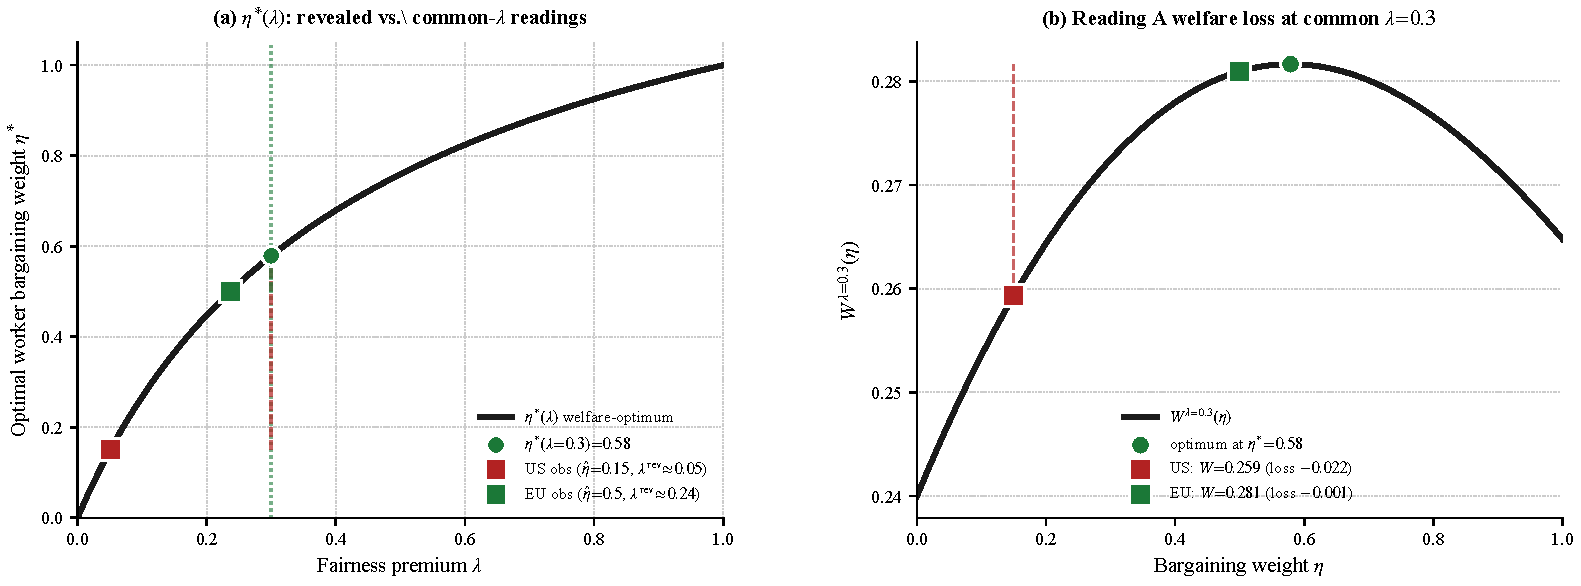
\includegraphics[width=0.86\linewidth]{sim_q7_eta_lambda.pdf}
\end{figure}

\vspace{-0.4em}
\textbf{Verdict.} Reading B accommodates observed cross-country bargaining heterogeneity; Reading A cannot. \textbf{The cross-country hours gap is a fairness-belief gap, recovered from observed bargaining institutions $+$ Q4/Q5 model structure.}
\end{frame}

% =========================================================================
\section{Synthesis}
% =========================================================================

% -------------------------------------------------------------------------
% Synthesis slide
% -------------------------------------------------------------------------
\begin{frame}{Synthesis: what the four channels deliver together}
\textbf{The chain.}
\begin{itemize}\setlength{\itemsep}{4pt}
    \item \textbf{Q1.} Tax wedges sign the EU--US hours gap correctly but leave a residual SD $\approx\!158$ hours --- a third of the entire DE--US gap.
    \item \textbf{Q4.} A binding hours cap pulls $h$ from $h^{\mathrm{firm}}$ toward $h^{\mathrm{soc}}$. Optimal at $\bar h\!=\!h^{\mathrm{soc}}$; welfare-improving on $(2h^{\mathrm{soc}}\!-\!h^{\mathrm{firm}},\,h^{\mathrm{firm}})$. \emph{Quantity instrument.}
    \item \textbf{Q5.} An encompassing union with bargaining weight $\eta$ delivers the same overshoot logic via wages: $dh/d\eta\!<\!0$, hump-shaped joint surplus, asymmetric pass-through under wage rigidity. \emph{Price instrument.}
    \item \textbf{Q7.} Confronting Q5 with US/EU coverage data + Saez--Stantcheva $\lambda$ recovers a fairness-belief gap $\Delta\lambda\!\approx\!0.19$ --- the missing variable in Q1's noisy cross-section.
\end{itemize}

\vspace{0.4em}
\textbf{What the comparative structure surfaces.} A result no single-channel treatment could produce: each country's institutional configuration is rationalised as the at-optimum response to its own fairness primitive. The EU--US hours gap is not an institutional misalignment to be corrected, but the equilibrium expression of cross-country preference heterogeneity.
\end{frame}

% -------------------------------------------------------------------------
% Thank-you / questions
% -------------------------------------------------------------------------
\begin{frame}
\centering
\vspace{1.5em}
{\Huge \textbf{Thank you}}\\[1.5em]
{\large Questions?}\\[2em]
{\small Full paper, companion appendix, replication scripts:}\\[0.4em]
{\footnotesize \texttt{github.com/AlessandroCaggia30/overworked-americans-takehome}}
\end{frame}

\end{document}
